\documentclass[11pt]{article}
\usepackage[utf8]{inputenc}
\usepackage[T1]{fontenc}
\usepackage[margin=1in]{geometry}
\usepackage{amsmath,amssymb}
\usepackage{booktabs}
\usepackage{array}
\usepackage{graphicx}
\usepackage{xcolor}
\usepackage{enumitem}
\usepackage{parskip}
\usepackage[colorlinks=true,linkcolor=blue!55!black,urlcolor=blue!55!black]{hyperref}

\definecolor{qcol}{RGB}{140,60,140}
\definecolor{boxbg}{RGB}{244,244,248}
\definecolor{trapcol}{RGB}{170,60,40}

% "your question" callout
\newcommand{\yourq}[2]{%
  \par\vspace{4pt}\noindent
  \textcolor{qcol}{$\leftarrow$ \textbf{your question:}
  \textit{``#1''}\; \textnormal{(#2)}}\par\vspace{4pt}}

% key-point block: rules above and below, indented both sides
\newenvironment{keybox}
  {\par\vspace{7pt}\noindent\hrule\vspace{5pt}%
   \begingroup\leftskip=1.2em\rightskip=1.2em\noindent\ignorespaces}
  {\par\endgroup\vspace{5pt}\hrule\vspace{7pt}}

\sloppy
\setlength{\emergencystretch}{3em}

\newcommand{\ds}{\mathrm{ds}}
\newcommand{\trap}{\textcolor{trapcol}{\textbf{[T]}}}

\title{\textbf{Everything Fourier in the paper}\\[4pt]
\large Personalized notes {\normalsize+} mastery quiz}
\author{Built from your own questions, sessions 2026-06-24 $\to$ 2026-08-13\\
\normalsize rev.\ 2026-08-13: plane/readout (\S\ref{sec:planereadout}),\\
\normalsize the $\ds \equiv N$ identity (\S\ref{sec:coord}), the mechanism-switch result (\S\ref{sec:prefix})}
\date{}

\begin{document}
\maketitle
\vspace{-2em}

\noindent\rule{\textwidth}{0.4pt}

\noindent\textbf{Source of truth:} \texttt{paper/main.tex} \S6.4 (\texttt{sec:story}),
\S6.5 (\texttt{sec:instruments}), App.~A.2--A.4 (\texttt{app:bg-fourier},
\texttt{app:bg-coord}, \texttt{app:bg-order}), App.~B (\texttt{app:procedures});
code \texttt{fourier\_suite.py}, \texttt{causal\_surgery.py}.

\noindent Sections end with a \textcolor{qcol}{purple callout} quoting what you
actually asked, so you can jump straight to the thing that confused you.

\noindent\rule{\textwidth}{0.4pt}

\tableofcontents
\newpage

\part*{Part I --- Notes}
\addcontentsline{toc}{section}{Part I --- Notes}

\section{The 60-second map}

There are \textbf{three separate Fourier instruments} in the paper. Most of your
confusion has been mixing them up. Keep them apart:

\begin{center}
\small
\begin{tabular}{@{}llp{5.4cm}l@{}}
\toprule
& \textbf{Instrument} & \textbf{Where it looks} & \textbf{Answers} \\
\midrule
\textbf{I1} & Period spectrum & \emph{inside} --- residual stream, L0--L24, final token
  & \emph{which} features exist, \emph{when} \\
\textbf{I2} & Output DFT over $\mathbb{Z}_9$ & \emph{outside} --- the 9 answer logits
  & coset only, or full residue \\
\textbf{I3} & Phase error / wedges (\texttt{atan2}) & \emph{inside}, scored in degrees
  & is the angle \emph{accurate enough} \\
\bottomrule
\end{tabular}
\end{center}

\begin{keybox}
I1 says ``the feature is \emph{there}.''\quad
I3 says ``the feature is \emph{good enough}.''\quad
I2 says ``the model \emph{emitted} it.''\\[2pt]
They are three different sentences about the same claim. I1 is Fig.~6 (left/middle/right),
I2 is the dotted line in Fig.~6, I3 is Fig.~5.
\end{keybox}

\section{Why a circle at all}

To output $N \bmod 9$ you need a quantity unchanged when you add $9$ to the input.
No linear function of $N$ does that --- linear functions are \emph{monotone},
residues are \emph{periodic}. The natural code is an \textbf{angle}:
\[
\theta = \frac{2\pi x}{T}, \qquad\text{represent } x \text{ by }
\big(\cos(2\pi x/T),\ \sin(2\pi x/T)\big).
\]
Add $T$ to $x$ and the pair is unchanged. So the pair carries \textbf{exactly
$x \bmod T$ and nothing else}. The 2-D subspace of the residual stream holding
that pair is a \textbf{period-$T$ plane}.

Two reasons networks actually use this code:
\begin{enumerate}[leftmargin=*,itemsep=2pt]
\item \textbf{Addition becomes rotation} --- angles add. A running total can be
accumulated by composing rotations, \emph{never materializing the integer total}.
\item A \textbf{linear} readout of the plane recovers the residue --- so a probe
can find it, and so can the model's own next layer.
\end{enumerate}

\textbf{Which periods a model has is a fact about its training data.} Pretraining
on base-10 text rewards predicting the next \emph{digit}, and the last digit of
$N$ is $N \bmod 10$. So periods $10$ and its divisors $2, 5$ (plus magnitude
periods like $100$) are useful. \textbf{Period 3 or 9 is never needed to continue
a decimal string.} That is the ``2--5-smooth basis'' of prior work, and P5/F1
confirm it in Pythia: value-periods $\{2,5,10,100\}$ decode at $R^2 \approx 0.95$
\emph{before any fine-tuning}, digit-sum periods $\{3,9\}$ at $R^2 < 0$.

\begin{keybox}
This is the whole reason the paper's law works. Local moduli ($m \mid 10^k$) are
free because pretraining already built their circle. Global moduli need a
\textbf{new circle} built from scratch.
\end{keybox}

\subsection{The plane and the readout, concretely}
\label{sec:planereadout}

``A linear readout of the plane recovers the residue'' packs three objects into
one clause. Here they are separately.

\textbf{The plane's basis: $u_{\cos}$ and $u_{\sin}$.} The ridge regression of
\S\ref{sec:i1} solves $W = (H^\top H + \lambda I)^{-1} H^\top t \in
\mathbb{R}^{1024 \times 2}$ --- two columns because there are two targets.
Column 1 holds the weights that predict $\cos(2\pi\,\ds/9)$ from $h$; after
QR-orthonormalization it is $u_{\cos}$. Column 2, predicting the sine, becomes
$u_{\sin}$. Each is just a probe weight vector: 1024 numbers, one per
residual-stream dimension, with the defining property
\[
u_{\cos} \cdot h \approx \cos(2\pi\,\ds/9), \qquad
u_{\sin} \cdot h \approx \sin(2\pi\,\ds/9).
\]
Geometrically: two perpendicular unit arrows in $\mathbb{R}^{1024}$. Every
activation $h$ casts a shadow on each; the shadow pair
$(c, s) = (u_{\cos}\!\cdot h,\; u_{\sin}\!\cdot h)$ is a point in the 2-D plane
they span, and if the circuit works that point sits at angle
$\theta = 2\pi\,\ds/9$. The other 1022 dimensions are invisible to the pair ---
that is what makes it a ``plane'': a 2-D window into a huge space. (Toy version:
if the stream were $\mathbb{R}^3$ with $h = (\cos\theta, \sin\theta,
\text{other})$, then $u_{\cos} = (1,0,0)$, $u_{\sin} = (0,1,0)$. In reality the
phase is smeared across arbitrary combinations of dimensions; the ridge fit
\emph{finds} the tilt.) Why two directions, not one? A single functional gives
$\cos\theta$ alone, which cannot tell $\theta$ from $-\theta$ --- the same
ambiguity \texttt{atan2} resolves, one level down. And why the QR step: the two
raw ridge columns are not guaranteed perpendicular or unit-length; the deletion
$h \mapsto h - UU^\top h$ only means ``remove the plane's component'' when $U$'s
columns are orthonormal.

\textbf{The readout: nine directions inside the plane.} For each candidate digit
$d \in \{0,\dots,8\}$, place a vector inside the plane at that digit's angle:
\[
w_d = \cos(2\pi d/9)\, u_{\cos} + \sin(2\pi d/9)\, u_{\sin},
\qquad
\text{score}_d = w_d \cdot h = \rho\,\cos\!\big(\theta - 2\pi d/9\big).
\]
That last identity is the whole thing: digit $d$'s score is a cosine of the gap
between where the clock hand points and where $d$'s direction points, so the
argmax picks the angularly nearest digit. Worked example, $\ds = 27$
($\theta = 0^\circ$):

\begin{center}
\begin{tabular}{@{}lccccc@{}}
\toprule
$d$ & 0 & 1 & 2 & 3 & 4 \\
\midrule
angle gap & $0^\circ$ & $40^\circ$ & $80^\circ$ & $120^\circ$ & $160^\circ$ \\
$\text{score}_d$ & $\mathbf{1.00}$ & $0.77$ & $0.17$ & $-0.50$ & $-0.94$ \\
\bottomrule
\end{tabular}
\end{center}

``Readout'' is not a metaphor: the $w_d$ are literally rows of the unembedding
matrix (or late-MLP weights composed into it), and argmax is what decoding does
anyway. Three things fall out of this construction:
\begin{enumerate}[leftmargin=*,itemsep=1pt]
\item \textbf{The wedges} (\S\ref{sec:atan2}) are the argmax's decision
boundaries --- halfway between adjacent $w_d$, $40^\circ$ apart for period 9.
Not an analogy; the boundary of these cosine scores.
\item \textbf{The output DFT measures exactly this readout}: with this wiring,
$\bar{p}(\Delta) \propto \cos(2\pi\Delta/9)$; if $\theta$ is pinned only mod
$120^\circ$ (coset knowledge), digits $d, d{+}3, d{+}6$ score identically and all
energy lands at $k=3$.
\item \textbf{The plateau is a wait, not a struggle}: constructing the plane is
hard; wiring nine dot products is trivial --- the oracle injection prices the
readout at 25--125 steps, $\sim$3\% of training.
\end{enumerate}

\emph{Caveat, as always:} ``a linear readout \emph{recovers} the residue'' is a
possibility claim --- the information is linearly available. Our probe finding
$R^2 = 0.93$ says such a readout exists; the model's own may read the same
subspace through different (non-orthogonal, scaled) vectors. The \emph{plane} is
the claimed object, not our particular pair of arrows in it.

\yourq{what does it mean a linear read out of the plane recovers the residue?
what plane? what readout?}{2026-08-12}
\yourq{what is u\_cos and u\_sin?}{2026-08-12}

\section{What $\cos/\sin(2\pi\,\ds/9)$ keeps, and what it throws away}
\label{sec:keeps}

The single most load-bearing fact in the mechanistic section, and the answer to
two of your questions at once.

\begin{itemize}[leftmargin=*,itemsep=2pt]
\item $\ds = 27$, $\ds = 36$, $\ds = 9$ $\Rightarrow$ \textbf{identical} $(\cos,\sin)$ pair.
\item The pair knows the \textbf{residue}. It does \textbf{not} know the \textbf{magnitude}.
\end{itemize}

So ``the converged model discards the digit-sum scaffold'' means:

\begin{center}
\begin{tabular}{@{}ll@{}}
\toprule
\textbf{fades} & the linear readout of the \emph{integer} $\ds$ \\
& $R^2: 0.98 \to 0.88 \to 0.63 \to 0.56$ (steps 250/2000/3500/6000, deep layers) \\
& \emph{i.e.\ the information distinguishing 27 from 36} \\
\midrule
\textbf{stays} & the periodic components $\cos/\sin(2\pi\,\ds/9)$, $R^2 \ge 0.93$ at convergence \\
& \emph{i.e.\ the residue} \\
\bottomrule
\end{tabular}
\end{center}

\textbf{No contradiction.} Computing a residue never requires materializing the
sum --- per-digit contributions can be accumulated \emph{directly as rotations}
on the period-9 circle. The converged network \textbf{keeps the phase and sheds
the count}.

\textbf{Which part of the figures shows this} --- it is deliberately split across
two figures with the same layers and the same checkpoints, different probe targets:
\begin{itemize}[leftmargin=*,itemsep=1pt]
\item what \textbf{fades}: Fig.~4 (\texttt{digitsum\_attn\_e1e2}), \textbf{middle row},
deep-layer curve $0.98 \to 0.56$
\item what \textbf{stays}: Fig.~6 (\texttt{fourier\_dynamics}), \textbf{left panel},
ds-period curves ending $0.97 / 0.93$
\end{itemize}

\yourq{does discarding digit sum means they no longer calculate digit sum? but
isn't that needed to calculate the mod?}{2026-07-28}
\yourq{not sure which part of figure suggests this}{2026-08-06}

\subsection*{Your later catch: isn't ``stays'' just the answer? (2026-08-12)}

Largely yes, at convergence --- and this is now conceded in the paper because you
forced it. The phase pair is a function of the residue alone $=$ a smooth
encoding of the answer; a model at 97.6\% accuracy must have the answer linearly
decodable at its final layer (the unembedding \emph{is} a linear readout), and
site consolidation puts the decision at L13--16, so high phase-$R^2$ there at
convergence is close to \emph{entailed} by behavior. The endpoint value of the
``stays'' half carries little independent weight. The independent content lives
in: (a) the \textbf{fade} --- nothing about task success requires deleting the
magnitude; (b) the \textbf{arrival timing}; (c) the \textbf{sibling-penalty run},
where behavior is a featureless ramp yet the spectra expose fine-first
construction; (d) two \textbf{dissociations} proving probe $\ne$ behavior: the
digit-sum donor holds a ds9 plane at $R^2 \ge 0.95$ with \emph{zero} mod-9
behavior, and the oracle-injection model sits at ceiling \emph{owning nothing}.

\yourq{we also said that the integer ds fades but integer ds mod 9 stays right?
isn't that just the answer thought? kinda weird..}{2026-08-12}

\section{Local vs.\ global periods --- and the identity you caught}
\label{sec:coord}

\emph{(Rewritten 2026-08-13. The original version of this section repeated the
paper's App.~A.3 claim that the measurement contrasts ``periodic in the digit
sum'' against ``periodic in $N$.'' You caught that this is wrong; the paper was
fixed the same day --- PROJECT\_STATE gotcha \#13.)}

Every prior Fourier analysis of LM arithmetic uses \textbf{single-token} operands
(GPT-2: $N \le 520$; Llama-3.1: $N \le 999$) and measures periodicity as a
function of the token's numeric value $N$. Our operands span up to \textbf{six
tokens}, which changes what the candidate \emph{periods} are. But one arithmetic
identity governs the labels:
\[
10 \equiv 1 \!\!\pmod 9 \;\;\Longrightarrow\;\;
\ds(N) \equiv N \!\!\pmod 9 \quad\text{(casting out nines; likewise mod 3)}.
\]
So for $T \in \{3, 9\}$, $\cos(2\pi\,\ds(N)/T) = \cos(2\pi N/T)$ \textbf{exactly,
for every operand} --- ``periodic in ds'' and ``periodic in $N$'' name the
\emph{same function}, and the probe target cannot distinguish a circuit that
tracks the value's residue from one that accumulates digits. (The code knows
this: \texttt{PERIODS} has no \texttt{("N", 9)} entry because it would be a
duplicate column.)

\begin{keybox}
\textbf{The honest contrast is between kinds of period, not coordinates:}
\textbf{local} periods ($T \mid 10^k$: 2, 5, 10, 100), computable from trailing
digits and rewarded by next-token prediction, versus \textbf{global} periods
(3, 9), functions of \emph{all} digits, which pretraining never needs. That
contrast is the paper's own digit-locality law, now visible inside the
representation. The ``ds'' label on the global periods marks the accumulation
\emph{hypothesis}; the evidence for the route is the prefix trace, the E2
aggregation dynamics, and the scaffold-donor transfer --- never the probe target
itself. Where the coordinates \emph{do} genuinely differ: the unwrapped integers
(ds $= 27$ vs.\ $N = 49059$ are different regression targets --- that licenses
the fade analysis), and the smooth periods (ds mod 2 $\ne$ $N$ mod 2).
\end{keybox}

Two corollaries worth having ready: mod 11 has the same structure ($10 \equiv -1$,
so the alternating sum $\equiv N$ mod 11), and mod 9 even the update rules
coincide --- the Horner step $v \mapsto 10v + d$ \emph{is} the rotation
$v \mapsto v + d$, so ``accumulate the digit sum'' and ``accumulate the running
value'' are the same circle operation. The honest name for the tracked object is
the \textbf{running residue phase}.

\yourq{in the fades vs stays, does residue here mean digitsum mod 9 or the pile
size mod 9? ig the answer is same but..}{2026-08-12}

\yourq{I'm not too sure if all papers apply ft the same way (some do it on the
logit, some on the weights, activation...) why do they do different stuff and how
are we doing dft in our case?}{2026-08-03}

\noindent\textbf{Answer.} They differ because of where the structure is legible in
\emph{their} setup. Nanda's grokking network is tiny and trained from scratch, so
the \textbf{weights/embeddings} are readable directly. The trig / activation-subspace
papers (Zhou 2406.03445, Kantamneni 2502.00873, 2505.05145) use \textbf{activations}
of single-token numbers. We do \textbf{both} --- activation-side (I1, ridge on
hidden states) \emph{and} output-side (I2, DFT on answer logits) --- and our twist
is the \textbf{period family}: probing global periods that only exist once
cross-token aggregation exists, in a regime where operands span many tokens.

\section{Instrument I1 --- the period spectrum (activations)}
\label{sec:i1}

Per checkpoint, per layer $\ell$, per coordinate $x$, per period $T$
(\texttt{fourier\_suite.py}):

\begin{enumerate}[leftmargin=*,itemsep=2pt]
\item Collect \textbf{final-position} residual vectors $h_i \in \mathbb{R}^{1024}$
for 2000 \textbf{training-pool} operands.
\item Targets $t_i = \big(\cos(2\pi x_i/T),\ \sin(2\pi x_i/T)\big)$.
\item Standardize $h$ per dimension; closed-form ridge
$W = (H^\top H + \lambda I)^{-1} H^\top t$, $\lambda = 10$, $W \in
\mathbb{R}^{1024\times 2}$. One batched GPU solve per layer.
\item Report \textbf{held-out} $R^2$ on 2000 unseen operands, averaged over the
cos/sin pair. \emph{This is what Fig.~6 plots.}
\item \textbf{QR-orthonormalize} $W$'s two columns $\to U_T^{(\ell)} \in
\mathbb{R}^{1024\times 2}$, the \textbf{period-$T$ plane} --- the object the
interventions later delete.
\end{enumerate}

\subsection*{Why ridge --- every symbol in step 3 (added 2026-08-13)}

The goal of the solve is $W$: two weight vectors, stacked as columns, such that
$h \cdot w_{\cos} \approx \cos(2\pi\,\ds/9)$ and
$h \cdot w_{\sin} \approx \sin(2\pi\,\ds/9)$ on \emph{held-out} operands ---
i.e.\ the tilt of the phase plane inside the 1024-dim stream, the object every
later measurement (R$^2$, \texttt{atan2}, deletion) is built from.
$H \in \mathbb{R}^{2000 \times 1024}$ is the design matrix (row $i$ = hidden
state of fit-operand $i$); $t \in \mathbb{R}^{2000 \times 2}$ holds the true
(cos, sin) pairs; we want $HW \approx t$. Least squares gives
$W = (H^\top H)^{-1} H^\top t$ --- but $H^\top H$ is a $1024 \times 1024$
covariance estimated from only 2000 correlated samples, so it has many
near-zero eigenvalues, and inverting it amplifies noise along barely-varying
directions: huge weights, memorized fit set, held-out $R^2$ craters. Adding the
penalty $\lambda \lVert W \rVert^2$ yields
$W = (H^\top H + \lambda I)^{-1} H^\top t$: the $+\lambda I$ lifts every
eigenvalue, the inverse is stable, no direction gets an absurd weight ---
slightly shrunken weights, much better generalization, and generalization is the
point, since the reported number is held-out. (Standardizing $h$ per dimension
first makes the uniform penalty fair across coordinates; the solve is batched
over all 25 layers as one GPU call.)

\textbf{Reading $R^2 = 1 - \mathrm{SS_{res}}/\mathrm{SS_{tot}}$:}
$1$ = perfect; $0$ = no better than predicting the mean;
\textbf{$R^2 < 0$ = the feature is genuinely absent}, not weak. This matters: at
the first checkpoints ds-period probes score $\approx -0.25$ (absent), not
$\approx 0.2$ (weakly present). The honest signature.

\textbf{Two standing warnings} (App.~A.1) --- both bite us later:
\begin{itemize}[leftmargin=*,itemsep=1pt]
\item Decodability is \textbf{presence}, not \textbf{use}. The mod-8 model retains
a decodable digit sum it demonstrably does not need.
\item Absence is evidence only against \textbf{linearly} readable presence, at the
probed layer and position.
\end{itemize}

\yourq{figure 4 shows that mod 8 seems to have similar or higher digit sum probe
signal, though it doesn't need it $\ldots$ so digit sum probe is not a safe way to
check if it's using digit sum info or not right?}{2026-07-21}

\noindent\textbf{Correct --- and the paper now concedes exactly this} in \S6.3's
caveat. No $R^2$ \emph{level} establishes use; the argument rests on within-model
\emph{change} and its \emph{timing}, and the arbiter of use is causal.

\subsection*{I1 results --- the numbers to remember}

\begin{center}
\small
\begin{tabular}{@{}lp{4.3cm}p{3.1cm}p{3.9cm}@{}}
\toprule
& \textbf{mod 9 (target)} & \textbf{mod 8 (control)} & \textbf{sibling-penalty} \\
\midrule
ds-period-3 & $-0.13 \to \mathbf{0.42}$@2250 $\to \mathbf{0.96}$@2500
  (plateau onset 2300) & flat-negative & stays $\approx 0$ through 3000 --- coset stage never forms \\
\addlinespace
ds-period-9 & flat until 3000, $\mathbf{0.77}$@3500 $\to 0.93$ (the snap)
  & flat-negative & $\mathbf{0.79}$@3500, \textbf{rises FIRST} \\
\addlinespace
$N$-periods $\{2,5,10,100\}$ & $\mathbf{0.93\text{--}0.95}$ from ckpt 1, then
  \textbf{decline to 0.52--0.57} & static \textbf{0.86--0.95 (retained)} & --- \\
\bottomrule
\end{tabular}
\end{center}

Two things to say out loud from that table:
\begin{enumerate}[leftmargin=*,itemsep=2pt]
\item The $N$-periods being high \emph{at the first checkpoint} is the pretrained
basis caught in the act, \textbf{before any task competence}.
\item Each model \textbf{keeps the basis it uses and discards the one it does
not} --- mod-9 sheds the value basis, mod-8 keeps it. Compression is visible
\emph{inside the periodic basis itself}, not just in the raw-sum probe.
\end{enumerate}

\section{Instrument I2 --- the output DFT over $\mathbb{Z}_9$}

The trick: our answers are \textbf{nine digit tokens}, so the \emph{answer space}
\textbf{is} $\mathbb{Z}_9$ regardless of tokenizer or vocab size. Tokenization
cannot interfere on the output side. (Nanda's logit analysis, transplanted.)

For each held-out example $i$ with true answer $y_i \in \{0,\dots,8\}$:
\begin{enumerate}[leftmargin=*,itemsep=2pt]
\item Take final-position logits, restrict to the nine digit-token ids
$\Rightarrow \ell_i \in \mathbb{R}^9$.
\item \textbf{Center}: $\ell_i \leftarrow \ell_i - \mathrm{mean}(\ell_i)$.
\item \textbf{Re-index by offset from the true answer}:
$p_i(\Delta) = \ell_i[(y_i + \Delta) \bmod 9]$.
So $\Delta = 0$ is the \textbf{correct} digit and $\Delta = 3, 6$ are its
\textbf{coset siblings}. \emph{Without this alignment, averaging across examples
with different answers would be meaningless.}
\item Average over examples $\Rightarrow \bar{p}(\Delta)$, a 9-point profile.
\item \textbf{DFT}: $F_k = \sum_\Delta \bar{p}(\Delta)\, e^{-2\pi i k \Delta/9}$,
$k = 0,\dots,4$; energies $e_k = |F_k|^2$.
\item \textbf{Coset fraction} $= e_3 / (e_1 + e_2 + e_3 + e_4)$ --- the DC term
$e_0$ is excluded.
\end{enumerate}

\textbf{Why $k=3$ is the coset:} a model that knows only the coset scores
$\Delta \in \{0,3,6\}$ equally. A profile with period 3 in $\Delta$ has
\emph{all} its non-DC energy at $k=3$.

\begin{keybox}
\textbf{Result (F2):} coset fraction $= \mathbf{1.000}$ for steps
\textbf{2250--3000} --- for \emph{exactly} the plateau steps, the output logits
are a \textbf{pure frequency-3 wave}. Falls to $\approx 0.45$ at the snap.
Sibling-penalty run: $\approx 0.000$ everywhere (manipulation check: the penalty
really did destroy coset expression).
\end{keybox}

\yourq{even dft period 3 and 9 show similar behavior as mod 3 acc and mod 9 acc.
hopefully that means smth internal}{2026-08-03}

\noindent Right instinct, but note the division of labor: \textbf{I2 is
\emph{not} internal} --- it is the output side, and it can only confirm what the
model \emph{emits}. The internal claim is I1 $+$ I3. The reason all three appear
in one figure is that the coincidence of \emph{internal arrival} with
\emph{external expression} is the point.

\section{Instrument I3 --- phase error, \texttt{atan2}, and the wedges}
\label{sec:atan2}

This is Fig.~5, the measurement that tests the wedge story \textbf{in its own
units} (degrees) rather than through a categorical probe.

\subsection*{Line by line, every symbol}

For a period $T \in \{3,9\}$ and one checkpoint:

\begin{enumerate}[leftmargin=*,itemsep=3pt]
\item On 2000 \textbf{training-pool} operands, collect final-position $h^{(\ell)}$
and ridge-fit $W^{(\ell)}$ predicting
$\big(\cos(2\pi\,\ds/T),\ \sin(2\pi\,\ds/T)\big)$ --- identical to I1.
\item Pick the \textbf{best layer} $\ell^\ast \in \{13,\dots,16\}$ by held-out $R^2$.
\item For each of 2000 \textbf{held-out} operands, form the predicted pair
$(\hat{c}, \hat{s}) = W^{(\ell^\ast)\top} h^{(\ell^\ast)}$ and decode the angle
\[
\hat{\theta} = \operatorname{atan2}(\hat{s}, \hat{c}).
\]

\textbf{\texttt{atan2} = the two-argument arctangent.} Given a point's $(x,y)$
coordinates it returns that point's angle on the \textbf{full} circle
$(-180^\circ, 180^\circ]$. Plain $\arctan(y/x)$ cannot: it returns only
$(-90^\circ, 90^\circ)$, so it confuses $(1,1)$ with $(-1,-1)$ --- the
\textbf{quadrant ambiguity}. \texttt{atan2} takes the two arguments separately and
keeps their signs, resolving it.
\emph{Mnemonic: it tells you where the clock hand points.}

\item True phase $\theta = 2\pi(\ds \bmod T)/T$. The angular error is
\[
\varepsilon = \hat{\theta} - \theta \quad\text{wrapped into } (-180^\circ, 180^\circ].
\]

\item A period-$T$ readout partitions the circle into $T$ classes of width
$360^\circ/T$, so the decode classifies \textbf{correctly iff}
$|\varepsilon| < 180^\circ/T$ --- the \textbf{class half-width}:

\begin{center}
\begin{tabular}{@{}cccc@{}}
\toprule
$T$ & classes & wedge width & \textbf{half-width (threshold)} \\
\midrule
3 & 3 & $120^\circ$ & $\mathbf{60^\circ}$ \\
9 & 9 & $40^\circ$  & $\mathbf{20^\circ}$ \\
\bottomrule
\end{tabular}
\end{center}

\item Fig.~5 plots, per checkpoint, the \textbf{fraction of held-out operands with
$|\varepsilon|$ below the half-width}.
\end{enumerate}

\subsection*{The result (P-C, textbook-clean)}

\begin{center}
\begin{tabular}{@{}lll@{}}
\toprule
& \textbf{crosses at} & \textbf{fraction within half-width} \\
\midrule
period-3 phase ($60^\circ$) & \textbf{plateau onset} &
  $0.34$@2000 $\to 0.70$@2250 $\to \mathbf{0.98}$@2500 \\
period-9 phase ($20^\circ$) & \textbf{the snap} &
  $0.15$@3000 $\to 0.76$@3500 $\to \mathbf{0.91}$@4250 \\
\bottomrule
\end{tabular}
\end{center}

\begin{keybox}
\textbf{Sanity check you should be able to reproduce on demand.} Before the plane
exists ($R^2 < 0$; e.g.\ period 9 before step 3250) the decoded angle is
\emph{meaningless}, so the fraction sits at chance $=$ the wedge's share of the
circle $= 2\times\text{half-width}/360^\circ = 1/T$:
$\approx 0.33$ for $T{=}3$, $\approx 0.11$ for $T{=}9$. Those are exactly the
pre-crossing baselines in the figure. Good figures have baselines you can predict
from first principles; this one does.
\end{keybox}

\yourq{too hard to understand.. what is atan2? explain line by line what each
symbol means plz}{2026-08-09}
\yourq{so we internally decoded the angle wedge they use? for mod 3 it was 120
degree? did we find anything else?}{2026-08-09}

\noindent\textbf{Yes --- that is precisely it.} We decoded the model's internal
clock hand and asked whether it lands in the right $120^\circ$ wedge (mod 3) or
the right $40^\circ$ wedge (mod 9). \textbf{And what else we found,} since you
asked:
\begin{enumerate}[label=(\alph*),leftmargin=*,itemsep=1pt]
\item the crossings coincide with the \emph{behavioral} events, not merely with each other;
\item the pre-crossing baselines land on their predicted chance values;
\item the \textbf{prefix trace} (\S\ref{sec:prefix});
\item the $N$-period \emph{decline} --- compression visible inside the periodic basis;
\item the digit-sum \textbf{donor} is already full of periodic structure (ds9 plane
$R^2$ 0.95--0.98 from step 1000, \emph{before any mod-9 training}), which
half-refuted our own pre-registration.
\end{enumerate}

\section{``The coset staircase is Fourier components arriving in order of robustness''}

You have asked about this sentence twice. Unpack it as \textbf{four claims}:

\begin{enumerate}[leftmargin=*,itemsep=2pt]
\item \textbf{``Fourier components''} --- the two things being built are the
period-3 plane and the period-9 plane. The stages of learning \emph{are} these
components.
\item \textbf{``arriving''} --- they appear at different times, and we can date
them: period-3 at 2250--2500, period-9 at 3500 (I1); confirmed in degrees (I3).
\item \textbf{``in order of''} --- the order is not arbitrary; it is the same in
every mod-9 run and it is \emph{reversible by intervention} (\S\ref{sec:spectral}).
\item \textbf{``robustness''} --- the ordering \emph{criterion} is \textbf{noise
tolerance}: not frequency, not difficulty.
\end{enumerate}

\textbf{The mechanism, in one picture.} Picture the model's running estimate of the
digit sum as a \textbf{point on a circle}. Early in training the aggregation
pathway (pooling digit features across all six numeral tokens) is half-built, so
that point \textbf{wobbles by tens of degrees}.

\begin{itemize}[leftmargin=*,itemsep=1pt]
\item A period-3 readout only needs the point in the right $120^\circ$ wedge
$\Rightarrow$ a wobble of tens of degrees is \textbf{tolerable}.
\item A period-9 readout needs the right $40^\circ$ wedge $\Rightarrow$ the same
wobble is \textbf{fatal}.
\end{itemize}

The coarse readout stays reliable at roughly \textbf{$3\times$ the noise level}
that already destroys the fine one.

\textbf{Plus the payoff is front-loaded:}
\begin{align*}
\text{uniform over 9 answers:} &\quad \ln 9 = 2.20 \text{ nats} \\
\big\downarrow\ \ \text{knowing only the coset} & \\
\text{uniform within correct coset:} &\quad \ln 3 = 1.10 \text{ nats}
\end{align*}

Knowing the coset is \textbf{exactly half of everything there is to gain} --- and
that half is reachable by the noise-tolerant machinery \emph{right now}. So greedy
gradient descent sees a \textbf{large, immediately realizable gradient} toward
period-3 and only a tiny one toward period-9. It builds the tolerant, high-reward
readout first $\Rightarrow$ accuracy locks at \textbf{exactly $1/3$} (the plateau)
$\Rightarrow$ then the fine one once the aggregate sharpens (the snap).

\begin{keybox}
\textbf{``payoff''} $=$ loss reduction per unit of phase precision purchased.\\
\textbf{``time cost''} $=$ f95, steps to reach 95\% of ceiling accuracy (3725 for
scratch mod 9).
\end{keybox}

\yourq{still not too sure what this means: The coset staircase is Fourier
components arriving in order of robustness}{2026-08-06}
\yourq{what does the payoff and time cost mean here?}{2026-08-08}

\section{Why this is the \emph{opposite} of spectral bias --- get this exactly right}
\label{sec:spectral}

You said \emph{``It looks like spectral bias to me, smaller period learning
faster.''} \textbf{That intuition is the one the appendix is written to kill.}
Do the frequency bookkeeping on $\mathbb{Z}_9$:

\begin{center}
\begin{tabular}{@{}p{4.0cm}p{5.6cm}p{3.1cm}@{}}
\toprule
\textbf{information} & \textbf{which Fourier mode on $\mathbb{Z}_9$} & \textbf{speed} \\
\midrule
\textbf{fine}\newline (the actual mod-9 residue) & the \textbf{fundamental, $k=1$} ---
  one slow cycle over nine residues & \textbf{lowest} frequency \\
\addlinespace
\textbf{coarse}\newline (the mod-3 coset) & the \textbf{$k=3$ harmonic} ---
  a wave three times faster & \textbf{higher} frequency \\
\bottomrule
\end{tabular}
\end{center}

\emph{Why:} a function of $r \bmod 3$ is periodic with period 3 on $\mathbb{Z}_9$,
so it is supported on modes whose $e^{2\pi i k r/9}$ has period 3
$\Rightarrow$ \textbf{$k$ a multiple of 3}.

\begin{keybox}
\textbf{Coarse $\ne$ low-frequency. The coset structure is the HIGH-frequency
component.} Spectral bias (Rahaman et al.: networks fit low frequencies first)
therefore \textbf{predicts the fine component first}. We observe the
\textbf{reverse}: $k=3$ arrives $\sim$1200 steps before $k=1$, and the output DFT
is pure frequency-3 throughout the plateau.
\end{keybox}

\textbf{Why the reversal:} here the ordering is set by \textbf{payoff per unit of
phase precision}, not by frequency.

\textbf{And we proved it causally.} The \textbf{sibling-penalty} run adds
$\lambda\big(p(r{+}3) + p(r{+}6)\big)$ at the answer position, penalizing the true
answer's two coset siblings. This \textbf{deletes no information}; it removes only
the coset's \emph{loss advantage}. Result:

\begin{itemize}[leftmargin=*,itemsep=1pt]
\item the plateau vanishes \textbf{behaviorally and internally} (coset fraction
$\approx 0$ everywhere; ds3 stays $\approx 0$);
\item \textbf{period-9 rises BEFORE period-3} (ds9 $0.79$ vs.\ ds3 $0.36$ at step
3500) --- \emph{the order spectral bias always predicted};
\item but learning is \textbf{48--85\% slower} (f95 5525/6875 vs.\ 3725).
\end{itemize}

\textbf{The clean statement:} the default spectral ordering is real, but it is
\textbf{overridden} by the coarse component's payoff asymmetry whenever the
objective offers one. Delete the payoff and the default reasserts itself. And
gradient descent takes the staircase \textbf{not because it must, but because it
is the fastest route available given nothing but the task's gradient}.

\yourq{It looks like spectral bias to me, smaller period learning faster than
finer 3 than 9? and not understand your explanation too much}{2026-08-03}

\section{The prefix trace (the accumulation signature)}
\label{sec:prefix}

The sharpest test of ``accumulate rotations, never build the integer sum.''

For $N = 49059$ tokenized as \texttt{" 49"}, \texttt{"059"}:
$\mathrm{prefix}_0 = 13$, $\mathrm{prefix}_1 = 27$. At each within-numeral
position $j$, probe the hidden state \emph{at that position} for the
\textbf{prefix phase} $(\cos,\sin)(2\pi\,\mathrm{prefix}_j/9)$ and for the
\textbf{full-sum phase}.

\textbf{Interpretation rule fixed in advance} (this is what makes it honest): a
\emph{single-token} position's prefix is a deterministic function of that token's
identity, so \textbf{any} model decodes it --- the mod-8 control does, at
$R^2 = 0.90$. Those positions are \textbf{excluded as confounded}. Only
\textbf{cross-token} positions bear on accumulation.

\begin{center}
\begin{tabular}{@{}lc@{}}
\toprule
\textbf{cell} & $R^2$ \\
\midrule
cross-token prefix phase, converged mod-9 & $\mathbf{0.95}$ \\
cross-token prefix phase, mod-8 control & $\mathbf{-0.27}$ \\
cross-token prefix phase, mod-9 \emph{pre-snap} & negative \\
\emph{full}-sum phase at early positions & $\mathbf{-0.16}$ (no anticipation) \\
\bottomrule
\end{tabular}
\end{center}

Within those scopes, the trace matches per-digit accumulation exactly.

\subsection*{The mechanism-switch test (P-D, run 2026-08-13): your hypothesis, tested}

You proposed a developmental alternative: maybe mid-training the model
\emph{materializes the count and wraps at readout} (``count-then-wrap''), and only
later learns the simpler running-rotation mechanism. Pre-registered as P-D and
run dense through the plateau$\to$snap window, with two new cells: the integer
\emph{prefix count} as a probe target, and \textbf{rotation increments} ---
decode $\hat{\theta}$ at consecutive numeral positions and compare
$\Delta\hat{\theta}$ against the predicted rotation $2\pi\,\ds(\mathrm{tok})/9$.

\textbf{H-count was killed} (its own kill condition): the cross-token count is
decodable at $0.98$ from step 250 --- but at $0.94$ in the \emph{mod-8 control}
too. It is the pretrained, magnitude-confounded feature, not a constructed
intermediate; it only fades, and never leads the phase in any task-specific
sense.

\textbf{H-rotate confirmed, 3/3, and the transition rule is now measured:}

\begin{center}
\small
\begin{tabular}{@{}lcccc@{}}
\toprule
& pre-snap & 3250 & 3500 & 6000 \\
\midrule
cross-token phase $R^2$ (L13--16) & $-0.25$ & $0.19$ & $0.78$ & $\mathbf{0.95}$ \\
median increment error & $\approx 90^\circ$ (chance) & $36^\circ$ & $10^\circ$ & $\mathbf{4.3^\circ}$ \\
frac.\ within $20^\circ$ & $0.10$ ($= 20/180$) & $0.33$ & $0.74$ & $\mathbf{0.95}$ \\
\bottomrule
\end{tabular}
\end{center}

Each token rotates the decoded clock hand by the predicted amount, to within
$\sim\!4^\circ$; the mod-8 control sits at chance at every checkpoint. Bonus,
half of which you predicted: the deep-layer (L13--16) count falls $0.98 \to 0.78$
with its \textbf{steepest drop exactly across the snap}, while the phase rises
there, and the count's best layer migrates L20--24 $\to$ L2--6. Refined story:
\emph{the count was inherited, never wrapped; the rotation circuit arrives whole
at the snap; the decision site evicts the count on its arrival.} Now Fig.~9 in
the paper (App.~B.4); scope: period-9 targets only --- the coset-stage
(period-3) version is untested.

\begin{center}
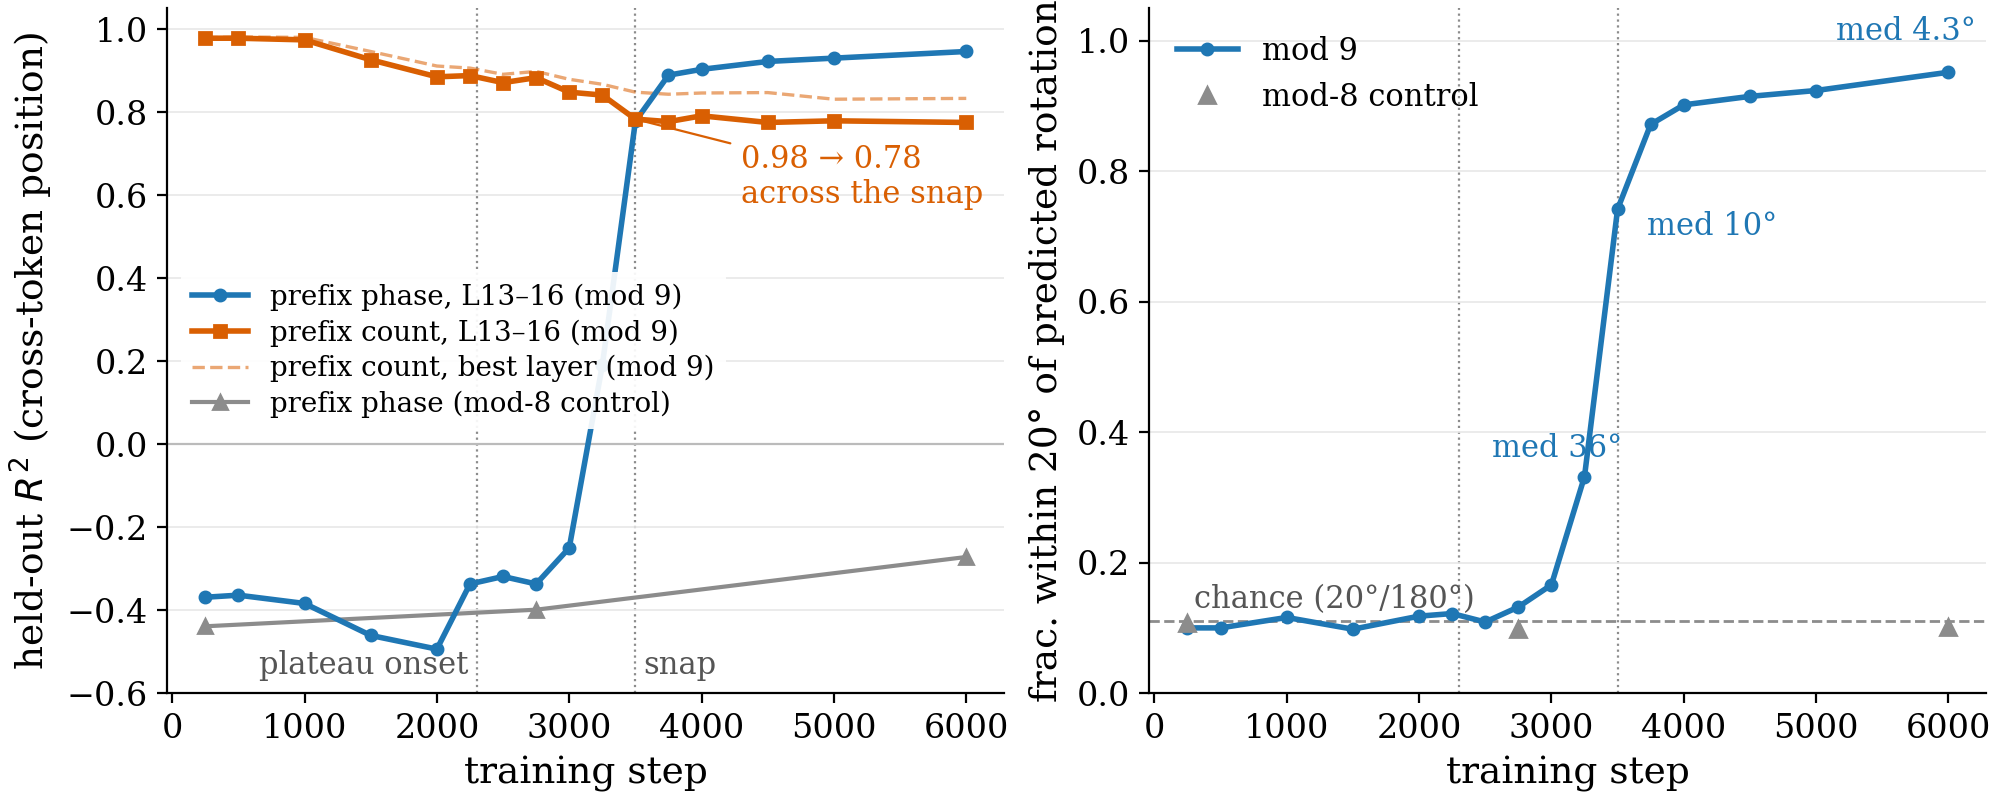
\includegraphics[width=\linewidth]{../new_result/plots/phase_switch.png}
\end{center}

\yourq{so are we claiming smth like the model keeps a mod 9 of the digitsum? for
ex, when it sees 357, it does 3 mod 9, 8 mod 9, and then 8 + 7 mod 9 which is
6?}{2026-08-13}
\yourq{cuz in earlier ckpt the digit sum was there right? so in mid point model
might have been doing digit sum, then mod 9, but the model learned a simpler
mechanism to just keep a running sum and doing mod 9 everytime}{2026-08-13}

\section{The deletions --- why we did them, and why all three are null}

You asked why we did ``the mean ablation and rank 8 deletion in the first place.''
It is an \textbf{escalating ladder}, each rung a sharper guess at where the answer
lives:

\begin{center}
\small
\begin{tabular}{@{}lp{4.6cm}p{4.6cm}l@{}}
\toprule
& \textbf{what was deleted} & \textbf{the guess being tested} & \textbf{result} \\
\midrule
\textbf{S1} & class-mean subspace (9 answer-class centroids $\Rightarrow$
  \textbf{rank $\le 8$} after centering) & ``the decision site holds 9 clusters;
  kill the cluster geometry, kill the readout'' & \textbf{null} \\
\textbf{S3} & the linear digit-sum direction (INLP) & ``kill the scaffold quantity''
  & \textbf{null} \\
\textbf{S4} & the period-9 plane itself (and ds3$+$ds9), L13--16, \emph{all
  positions} & ``kill the periodic code F1 \emph{proved} exists'' & \textbf{null} \\
\bottomrule
\end{tabular}
\end{center}

\noindent(S1 also projected only the \emph{final position} --- one stated reason
it failed.)

\textbf{Mechanics (App.~B.3):} register a forward hook on
\texttt{gpt\_neox.layers[L-1]} --- the module whose output \emph{is}
\texttt{hidden\_states[L]}, since index 0 is the embeddings (that off-by-one is a
real trap, and it is in the quiz) --- and replace its output by
$h \mapsto h - U U^\top h$. Control: a \textbf{dimension-matched random plane} (QR
of a Gaussian). Four \textbf{consecutive} layers (13--16), so the immediately
downstream layer cannot re-derive the deleted phase from the same-position residual.

\textbf{What the nulls mean, at the right strength:} they do \textbf{not} falsify
the account. Each is \textbf{scoped} --- by fit position, by untouched layers, by
re-import from other positions via attention. The cumulative reading we keep:

\begin{keybox}
\textbf{No low-rank, single-position cut we found removes the learned mechanism.}
Training distributes it into redundant copies.
\end{keybox}

Two consequences the paper draws honestly:
\begin{enumerate}[leftmargin=*,itemsep=2pt]
\item Site consolidation is an \textbf{observational} fact about where the decision
is first \emph{readable} --- \textbf{not} a causal bottleneck.
\item The decisive causal evidence comes from the \textbf{opposite direction ---
adding} the structure: the \textbf{oracle injection} (inject the phase plane into
the residual stream $\Rightarrow$ task learnable in \textbf{25--125 steps}, so
readout is $\sim$3\% of from-scratch training and the plateau is almost entirely
\emph{the wait for the feature to exist}), and the \textbf{sibling-penalty} order
inversion (\S\ref{sec:spectral}).
\end{enumerate}

\yourq{the fourier appendix is so hard I'm not sure what's going on, why we did
the mean ablation and rank 8 deletion in the first place}{2026-08-06}

\section{Mentor-proofing: the four things you will be asked}

\begin{enumerate}[leftmargin=*,itemsep=4pt]
\item \textbf{``Isn't this just spectral bias?''} $\to$ No, and we did the
bookkeeping: coarse $= k{=}3 =$ \emph{high} frequency. Spectral bias predicts the
opposite of what we see. The sibling-penalty run \emph{recovers} the spectral-bias
order once the payoff is removed. (\S\ref{sec:spectral})

\item \textbf{``Probes only show presence.''} $\to$ Conceded explicitly in the
paper; the mod-8 model is our own counterexample. The argument rests on
within-model \emph{change} and \emph{timing}; the causal arbiters are injection and
sibling-penalty, not probing.

\item \textbf{``Your ablations were all null --- doesn't that sink it?''} $\to$
Scoped nulls, stated as a characterization (redundant distributed copies), not
hidden. Causal weight comes from \emph{adding}, not deleting.

\item \textbf{``You claim the model discards the digit sum but needs it.''} $\to$
Residue $\ne$ count. The phase stays ($R^2 \ge 0.93$), the magnitude fades
($0.98 \to 0.56$), and accumulation as rotations never needs the integer. The
prefix trace confirms it --- and the increment test now shows the rotation itself,
median error $4.3^\circ$. (\S\ref{sec:keeps}, \S\ref{sec:prefix})

\item \textbf{``Your ds-period probe is just probing the answer --- ds mod 9
\emph{is} N mod 9.''} $\to$ Conceded and fixed (we caught it 2026-08-12; App.~A.3
rewritten): the probe target is the same function under both labels, and the
measured contrast is local vs.\ global \emph{periods}. The route claim rides on
the prefix trace, E2 aggregation, and donor transfer. And ``phase stays at
convergence'' is near-entailed by accuracy + consolidation --- the independent
content is the fade, the sibling-penalty order inversion, and the two
dissociations. (\S\ref{sec:coord}, \S\ref{sec:keeps})

\item \textbf{``Did you reverse-engineer the circuit?''} $\to$ Calibrated answer:
we identified the algorithm and verified its \emph{states} (prefix trace), its
\emph{update rule} (increments, $4.3^\circ$), their \emph{arrival times}, and
killed the pre-registered alternative (count-then-wrap). The head/MLP-level
implementation --- who does the rotating --- is open; head ablation and
cross-checkpoint patching are the listed follow-ups. (\S\ref{sec:prefix})
\end{enumerate}

\section{Five-line summary you can say from memory}

\begin{keybox}
Pretraining gives Pythia a base-10 periodic number basis --- the local periods
2, 5, 10, 100, and \textbf{no} period 3 or 9. Fine-tuning on mod 9 must build
\textbf{new global-period circles} (periods 3 and 9, functions of every digit,
tracked as a running residue phase), and it
builds them in order of \textbf{noise-robustness}, not frequency: the $120^\circ$
period-3 wedge survives the half-built aggregator's phase wobble and pays half the
total loss reduction ($\ln 9 \to \ln 3$), so it arrives first and pins accuracy at
$1/3$; the $40^\circ$ period-9 wedge arrives only when the aggregate sharpens, and
that is the snap. We watched both arrive (period spectrum), watched the answer
logits go pure frequency-3 for exactly the plateau (output DFT), measured the
phase error in degrees and saw each cross its wedge threshold at its own
behavioral event (\texttt{atan2}/wedge test), and inverted the order causally by
deleting the coarse component's payoff.
\end{keybox}

\newpage
\part*{Part II --- Mastery quiz}
\addcontentsline{toc}{section}{Part II --- Mastery quiz}

Same house style as \texttt{quiz\_paper.md}: answer any subset at any length,
grading with explanations follows. Questions marked \trap{} are traps --- phrased
the way a skeptical mentor would phrase them, and the naive answer is wrong.

\section*{Round 1 --- Warm-up (can you state the objects)}
\addcontentsline{toc}{subsection}{Round 1 --- Warm-up}
\begin{enumerate}[leftmargin=*,itemsep=4pt]
\item Why can no linear function of $N$ compute $N \bmod 9$? Give the one-word
property that fails.
\item What exactly does the pair $(\cos(2\pi\,\ds/9), \sin(2\pi\,\ds/9))$ know
about $\ds$, and what does it not know? Give two concrete values of $\ds$ it cannot
tell apart.
\item Pythia has period-2, 5, 10, 100 structure before any fine-tuning but no
period-3 or period-9. Explain \emph{from the pretraining objective} why that
specific set.
\item Name the three Fourier instruments, and for each: where it looks
(inside/outside) and the one question it answers that the other two cannot.
\end{enumerate}

\section*{Round 2 --- The wedge account}
\addcontentsline{toc}{subsection}{Round 2 --- The wedge account}
\begin{enumerate}[leftmargin=*,itemsep=4pt,start=5]
\item A period-3 readout tolerates $\sim 3\times$ the angular noise a period-9
readout tolerates. Where does the ``$3\times$'' come from --- give the two wedge
widths and the two thresholds.
\item Compute the loss drop from ``uniform over 9 answers'' to ``uniform within the
correct coset,'' in nats. What fraction of the \emph{total} available reduction is
that, and why does that fraction matter for the ordering argument?
\item \trap{} ``Your staircase is just spectral bias --- the network fits the easy,
smooth, low-frequency thing first.'' Rebut precisely: which Fourier mode on
$\mathbb{Z}_9$ carries the \emph{coarse} information, which the \emph{fine}, which
is faster, and what does spectral bias therefore predict for us?
\item The sibling-penalty run is the causal half of Q7. State (a) what it adds to
the loss, (b) why it deletes no information, (c) the two spectral outcomes
observed, (d) the cost in f95, and (e) why (d) is the sentence that makes the whole
staircase story interesting rather than trivial.
\end{enumerate}

\section*{Round 3 --- Procedures (could you re-run it from memory)}
\addcontentsline{toc}{subsection}{Round 3 --- Procedures}
\begin{enumerate}[leftmargin=*,itemsep=4pt,start=9]
\item Walk through the output DFT over $\mathbb{Z}_9$ in six steps. Be specific
about step 3 (the re-indexing) and say \emph{why} averaging would be meaningless
without it.
\item Why is $e_3$ the coset energy and not $e_1$? And why is the coset fraction's
denominator $e_1{+}e_2{+}e_3{+}e_4$ rather than $e_0{+}\dots{+}e_4$?
\item The output DFT is called ``vocab-independent'' / ``where tokenization cannot
interfere.'' Explain why that is true here, and why the same claim would
\emph{not} hold for the activation-side probes.
\item Define \texttt{atan2} and state the exact failure of $\arctan(\hat{s}/\hat{c})$
it fixes. Then walk the phase-error measurement from hidden state to ``fraction
within half-width,'' naming every symbol.
\item Before the period-9 plane exists, Fig.~5's period-9 curve sits at
$\approx 0.11$. \textbf{Derive} that number from the wedge geometry --- do not
recall it.
\item In period-plane estimation: why standardize $h$ per dimension, why ridge with
$\lambda = 10$ rather than plain OLS, why fit on train-pool but score on held-out,
and what does a \textbf{negative} held-out $R^2$ tell you that a small positive one
does not?
\item What is the QR step for? What object does it produce, and which later
experiment consumes that object?
\end{enumerate}

\section*{Round 4 --- Reading our own results}
\addcontentsline{toc}{subsection}{Round 4 --- Reading our own results}
\begin{enumerate}[leftmargin=*,itemsep=4pt,start=16]
\item From the F1 table: the $N$-coordinate periods start at 0.93--0.95 at the
\emph{first} checkpoint and decline to $\sim$0.55 in mod 9, but stay 0.86--0.95 in
mod 8. State both halves of what that pair of facts demonstrates.
\item Coset fraction $= 1.000$ for steps 2250--3000 exactly. What does the value
\emph{1.000} (rather than, say, 0.7) rule out about the model's state during the
plateau?
\item \trap{} ``Deep-layer digit-sum $R^2$ falls $0.98 \to 0.56$, so the converged
model stops using digit sums --- but it needs them to compute mod 9. Your story is
incoherent.'' Resolve it, and name the two figures (and which curve in each) that
hold the two halves of the resolution.
\item The prefix trace reports cross-token prefix-phase $R^2 = 0.95$ in mod 9 and
$-0.27$ in mod 8 --- but \emph{single}-token positions decode at 0.90 even in
mod 8. Why are single-token positions excluded, and why does it matter that we
fixed that rule \emph{before} reading the numbers?
\item What did the \texttt{fourier2} donor sweep predict, and how was the prediction
half-refuted? What does the actual result (ds9 plane $R^2$ 0.95--0.98 in the
digit-sum donor from step 1000, coset fraction $\approx 0$) say about \emph{why}
the scaffold donor gives an $18.6\times$ speedup?
\end{enumerate}

\section*{Round 5 --- Synthesis \& mentor defense}
\addcontentsline{toc}{subsection}{Round 5 --- Synthesis \& mentor defense}
\begin{enumerate}[leftmargin=*,itemsep=4pt,start=21]
\item \trap{} ``All three of your ablations returned null. Doesn't that mean you
haven't shown the periodic planes are used at all?'' Give the honest answer: what
the nulls are scoped by, the one characterization we keep, and where the causal
weight actually comes from instead.
\item In \texttt{causal\_surgery.py} the hook for \texttt{hidden\_states[L]} goes on
\texttt{gpt\_neox.layers[L-1]}. Explain the off-by-one, and explain why S4 ablates
four \emph{consecutive} layers rather than one.
\item S1 projected only the final position; S4 projected all positions. Name a
concrete mechanism by which the S1 design could return null \emph{even if} the
class-mean subspace were genuinely load-bearing.
\item The oracle injection makes the task learnable in 25--125 steps. Convert that
into the paper's claim about what the plateau \emph{is}, with the percentage. Then
state the control's second half and why it is the more alarming result.
\item Prior Fourier work on LM arithmetic restricts to single-token operands.
State our methodological delta in one sentence --- and say what it is
\emph{not}: why ``a delta of coordinate'' overstates it for periods 3 and 9
(state the identity), and what the honest contrast is instead.
\item (Bonus, synthesis) Give the five-line account: from ``what pretraining
supplies'' to ``why the snap happens when it does,'' using only these terms:
periodic basis, global period, aggregation pathway, wedge width, payoff. No
numbers needed --- but every clause should be one you could defend with a
measurement if pressed.
\end{enumerate}

\section*{Round 6 --- The identity \& the switch (added 2026-08-13)}
\addcontentsline{toc}{subsection}{Round 6 --- The identity \& the switch}
\begin{enumerate}[leftmargin=*,itemsep=4pt,start=27]
\item Prove $\ds(N) \equiv N \pmod 9$ in one line. Then state its two
consequences for our instruments: what the ds9 probe can never show, and which
three pieces of evidence carry the route claim instead.
\item \trap{} ``Your `phase stays at convergence' result is a tautology --- any
accurate model has its answer decodable.'' How much of this is right? Say
exactly which half of fades/stays is near-entailed and by what, and name the four
places the independent content lives.
\item Mod 9, show that the Horner update $v \mapsto 10v + d$ and the digit-sum
update $v \mapsto v + d$ are the same operation on the circle. What does this
make the honest name of the tracked quantity, and which distinction does it
render empty?
\item State H-count and H-rotate, and the two cells that discriminate them.
Which kill condition fired, and on what evidence? (Careful: the cross-token
count \emph{was} present while the phase was absent --- why did that not confirm
H-count?)
\item The increment test's pre-snap fraction sits at $0.10$. \textbf{Derive}
that chance level from the acceptance window --- and explain what the converged
value of $0.95$ with median error $4.3^\circ$ establishes that the prefix trace
alone could not.
\item (Synthesis) ``Discards the scaffold'' has now been sharpened three times:
by the identity (\S\ref{sec:coord}), by the eviction timing, and by the kill of
count-then-wrap. Give the final one-paragraph version of the story --- inherited
vs.\ built, wrapped vs.\ never-wrapped, and what happens at the snap.
\end{enumerate}

\end{document}
